\section{Deliberate Score Grouping}
\label{sec-roundingoff}

We now consider whether the deliberate use of tied scores -- which
might allow efficiency improvements in the underlying search system
-- has a discernible effect on retrieval effectiveness.

\myparagraph{Score Approximation}

Scoring documents using modern similarity computations involves
non-trivial amounts of arithmetic, especially if phrase components or
term proximity components are being used.
Regimes such as WAND {\citep{bchsz03cikm}} seek to minimize the
number of documents scored, while still giving rise to exactly the
same ranking for the top-$k$ documents, an approach that meets the
requirements for being {\emph{rank safe to depth $k$}}.
That is, the WAND process ensures that all of the documents in the
first $k$ positions of the ranking are in their ``right'' positions
in the ranking that is generated, but makes no such guarantee for
documents beyond depth $k$.
This is a relatively stringent requirement, and other
computation-pruning techniques might also be considered that provide
alternative and more flexible trade-offs.

In particular, we now consider the following weaker requirement: that
each document must be scored in a manner that guarantees that it is
in the correct {\emph{band}} of the ranking, where the bands are
defined geometrically based on a parameter $\rho>1$.
More precisely, let $b_1=1$, and thereafter let
$b_{g+1}=\lceil{\rho\cdot b_g}\rceil$.
The $g$\,th group, for $g\ge1$, spans the ranks from $b_g$ to
$e_g=b_{g+1}-1$ inclusive.
For example, if $\rho=2$, then the bands are $[1\ldots1]$,
$[2\ldots3]$, $[4\ldots7]$, and so on; and if (say) $\rho=1.62$ (the
golden ratio) the bands are $[1\ldots1]$, $[2\ldots3]$, $[4\ldots6]$,
$[7\ldots11]$, and so on, with widths given by the Fibonacci
sequence.
The smaller the value of $\rho$, the smaller the group is that spans
any given position in the ranking, and the nearer the approximate
ranking is to the ``true'' and exact ranking.
In the limit, as $\rho$ approaches $1$, the retrieval system is
obliged to place each of at its final ``correct'' position; that is,
$\rho=1$ corresponds to a ``full'' computation in which all document
relationships are finalized.
But when $\rho>1$, we allow the retrieval system to economize on its
computational costs and return bands of documents $[b_g\ldots e_g]$,
with equal scores assumed within each band.

\myparagraph{Worst-Case Bounds}

It is straightforward to show that the first group containing more
than one document starts at rank $v=b_v=1+\lfloor{1/(\rho-1)}\rfloor$.
That fact implies that the approximate scoring mechanism is rank-safe
to depth $v-1$, and more generally, allows bounds on the imprecision
in scores to be computed.
For example, consider the metric reciprocal rank (RR).
With the $v$\,th group the first one with multiple documents in it,
the maximum loss of score that can arise relative to the original is
given by
\[
	\Delta\mbox{RR} = \frac{1}{b_v} -
		\frac{1}{e_v-b_v+1}\sum_{k=b_v}^{e_v} \frac{1}{k} \,,
\]
where the bound arises because the worst situation is when the
original run has its first relevant document at rank $b_v$, and no
other document in that group is relevant.
Table~\ref{tbl-bounds} gives some $\Delta$RR values; when $\rho\le2$,
all are less than $0.1$.


\begin{table}[t]
\centering
\renewcommand{\tabcolsep}{0.5em}
\begin{tabular}{l c ccc}
\toprule
\multirow{2}{*}{$\rho$}
	&& \multicolumn{3}{c}{Metric}
\\
\cmidrule{3-5}
	&& RR
		& RBP0.5
			& RBP0.85
\\
\midrule
1.1
	&& 0.0038
		& 0.0002
			& 0.0087
\\
1.2
	&& 0.0119
		& 0.0052
			& 0.0231
\\
1.4
	&& 0.0417
		& 0.0429
			& 0.0482
\\
2.0
	&& 0.0833
		& 0.1016
			& 0.0971
\\
\bottomrule
\end{tabular}

\caption{Worst-case metric score differences associated with geometric
grouping of documents in runs, controlled by parameter $\rho$.
\label{tbl-bounds}}
\end{table}

It is also possible to compute worst-case differences for rank-biased
precision (RBP, see {\citet{mz08acmtois}}).
In the case of RBP, the maximum difference $\Delta$RBP arises when a
run has relevant documents at every rank in the first half of each
group, and non-relevant documents at every rank in the second half of
each group.
Each of the relevant documents in the multi-item groups then loses a
fraction of its weighting, because it gets ``smeared'' across the
whole of the group.
{\alistair{Need to think about this, argument should probably be on
weight being half, not number.}}
Table~\ref{tbl-bounds} includes $\Delta$RBP differences for two
values of the RBP parameter $p$.
Recall-based metrics such as average precision (AP) cannot be
analyzed as readily, because the highest metric score might not
correspond to the largest number of relevant documents.
Experimental results showing that practice that AP has less
divergence of scores than does RBP are presented in the next
subsection.


\myparagraph{Effectiveness Score Differences in Practice}

Given these worst-case bounds, the next question we ask is this: to
what extent does an allowance for rank-based score imprecision affect
effectiveness scores in practice?
To respond to this question, we again make use of the 1998 TREC7
resources, taking the same system runs as were already examined in
Section~\ref{sec-trecimpact}, and for each run, mapping it to a set
of equivalent banded runs based on a set of $\rho$ values, with the
documents ranked in band $g$ in each of those runs assigned a
synthetic score of $1/g$.
The original system scores that were part of the TREC7 data were
ignored as the grouping operation was being carried out, and original
file order was used as the reference point for each run.
As in Section~\ref{sec-trecimpact}, five runs in which the scores and
the assigned ranks were inconsistent were removed from the
experiment.

\begin{figure}[t!]
\centering
\subfloat[RR\label{fig-score-variation-rr}]{%
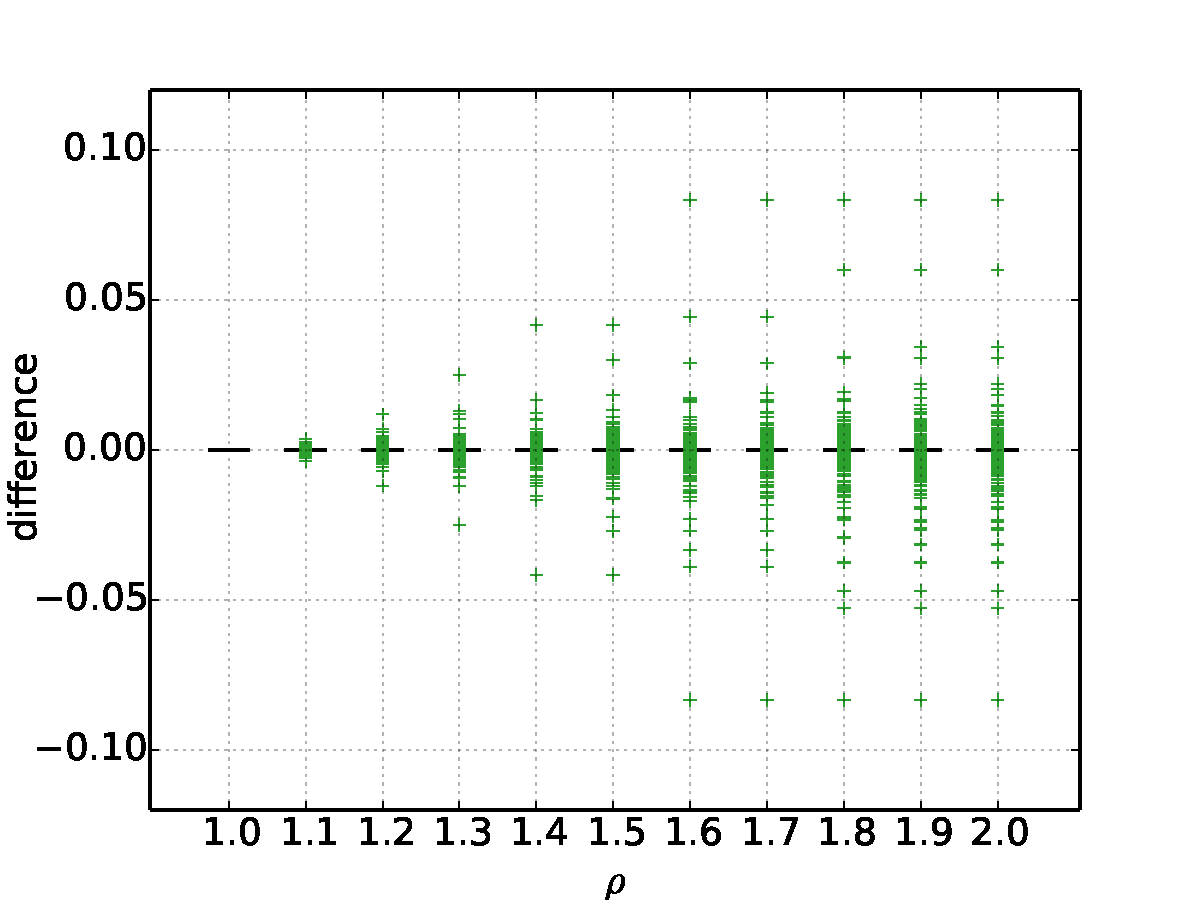
\includegraphics[width=0.49\textwidth]{figs/fig-score-variation-rr.pdf}
}
\subfloat[RBP0.5\label{fig-score-variation-rbp50}]{%
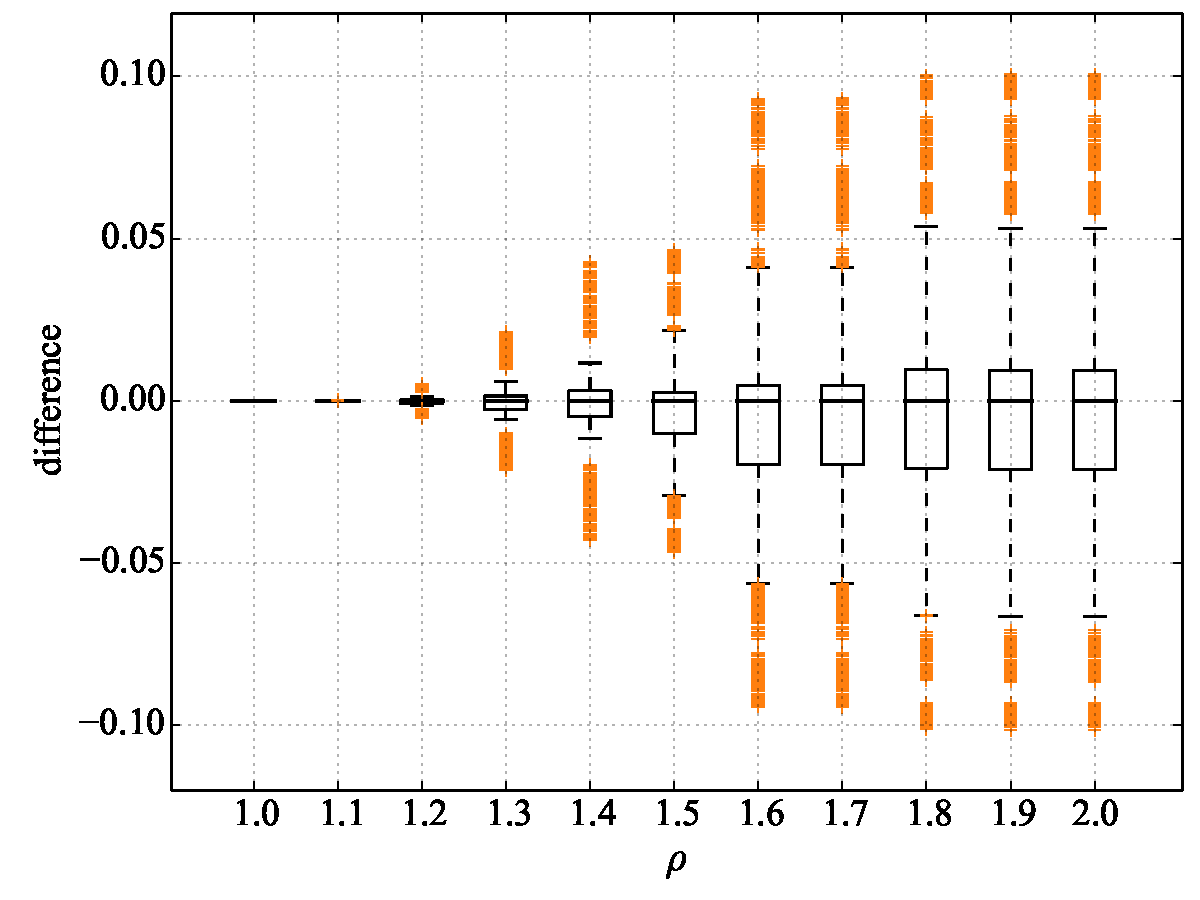
\includegraphics[width=0.49\textwidth]{figs/fig-score-variation-rbp50.pdf}
}
\\
\subfloat[RBP0.85\label{fig-score-variation-rbp85}]{%
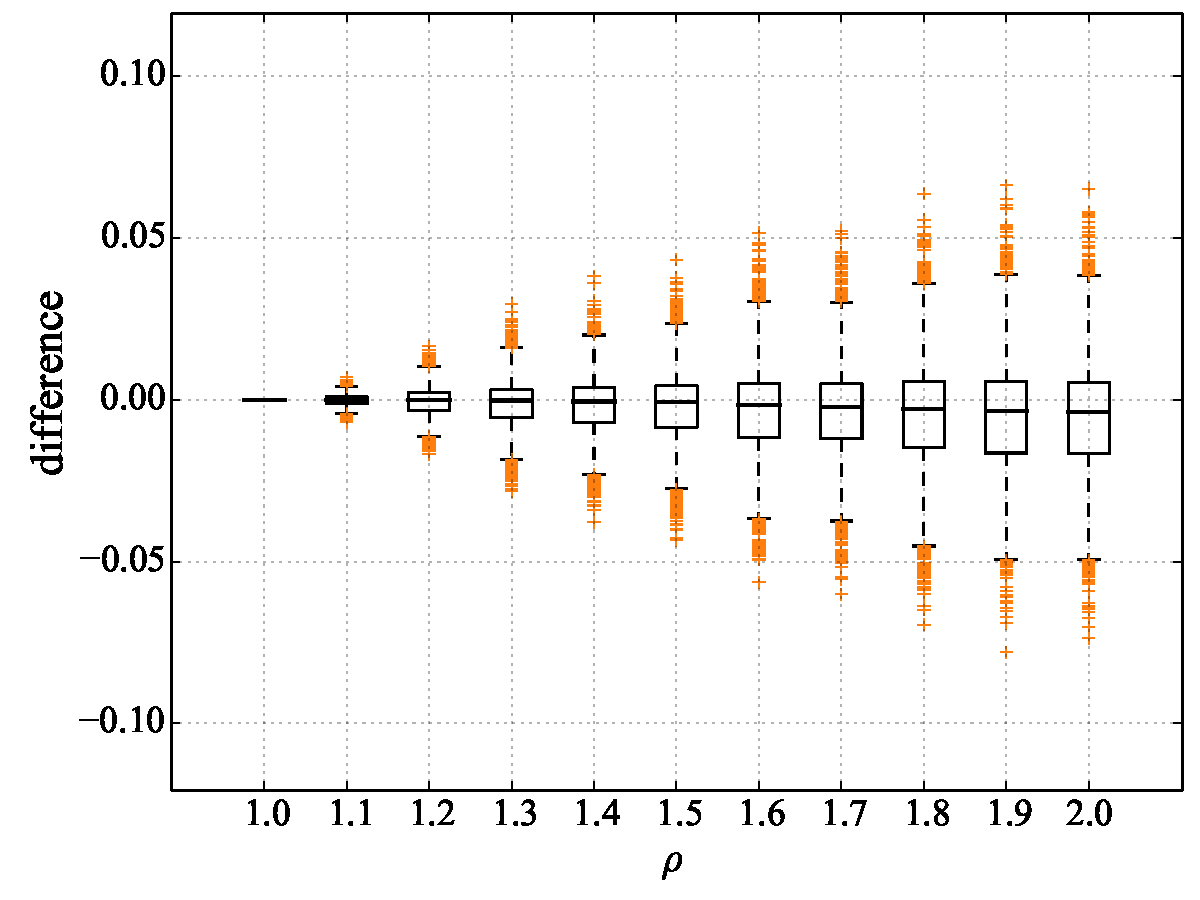
\includegraphics[width=0.49\textwidth]{figs/fig-score-variation-rbp85.pdf}
}
\subfloat[AP\label{fig-score-variation-ap}]{%
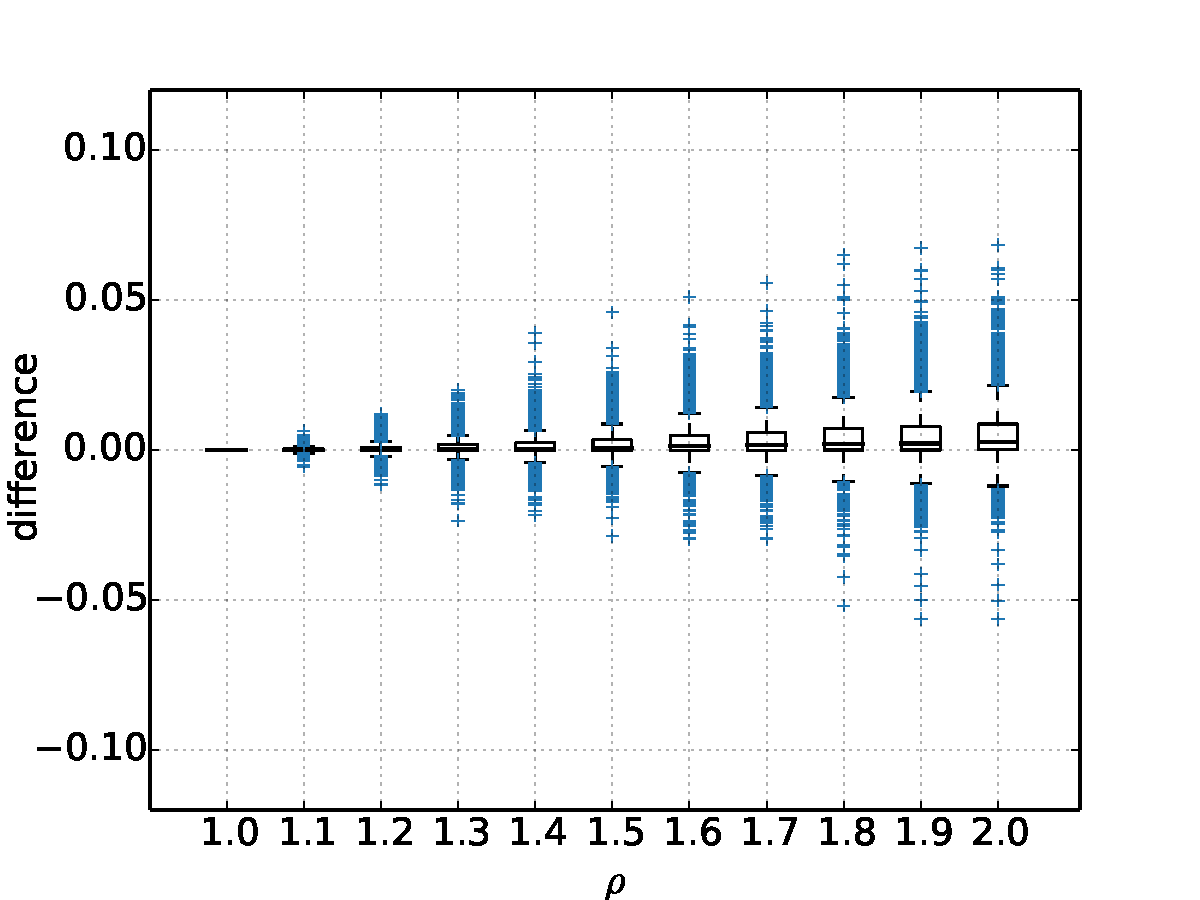
\includegraphics[width=0.49\textwidth]{figs/fig-score-variation-ap.pdf}
}
\caption{Variation in metric effectiveness score across a set of $98$
runs and $50$ topics (that is, there are $50 \times 98$ points
plotted in each column), as a function of $\rho$, for four different
retrieval effectiveness metrics.
The colored points beyond the whiskers represent outliers that are
below the $10$-percentile or above the $90$-percentile of that
distribution.
\label{fig-score-variation}}
\end{figure}

Figure~\ref{fig-score-variation} shows the results of this
experimentation, plotted as a sequence of box-whisker elements using
four different effectiveness metrics and eleven values of $\rho$.
In all cases the score difference calculated is the
across-permutations computation that was illustrated in
Section~\ref{sec-ties} when applied to the deliberately-tied
rankings, subtracted from the score the same metric achieves on the
original submitted ranking for that same topic.
(We used a modified version of {\tt{trec\_eval}} to ensure that this
was done consistently.)
We also followed standard protocols and assumed that unjudged
documents were not relevant for the purposes of scoring the runs.

Figure~\ref{fig-score-variation} shows that the average score
variation arising from the banding process is very small, and that
there are nearly as many rankings that gain from the approximation
process as there are that lose from it.
The two shallow metrics (RR and RBP$0.5$) are more affected than the
two deep-evaluation metrics (RBP$0.85$ and AP), and show clear
patterns of behavior.
In particular, note that difference in the RBP$0.5$ as $\rho$ shifts
from $1.5$ to $1.6$, and the second group expands from containing one
document to two documents.
In all cases in which $\rho\le2$ the first group contains only a
single document.


\begin{figure}[t!]
\centering
\subfloat[RR\label{fig-rho-p-value-rr}]{%
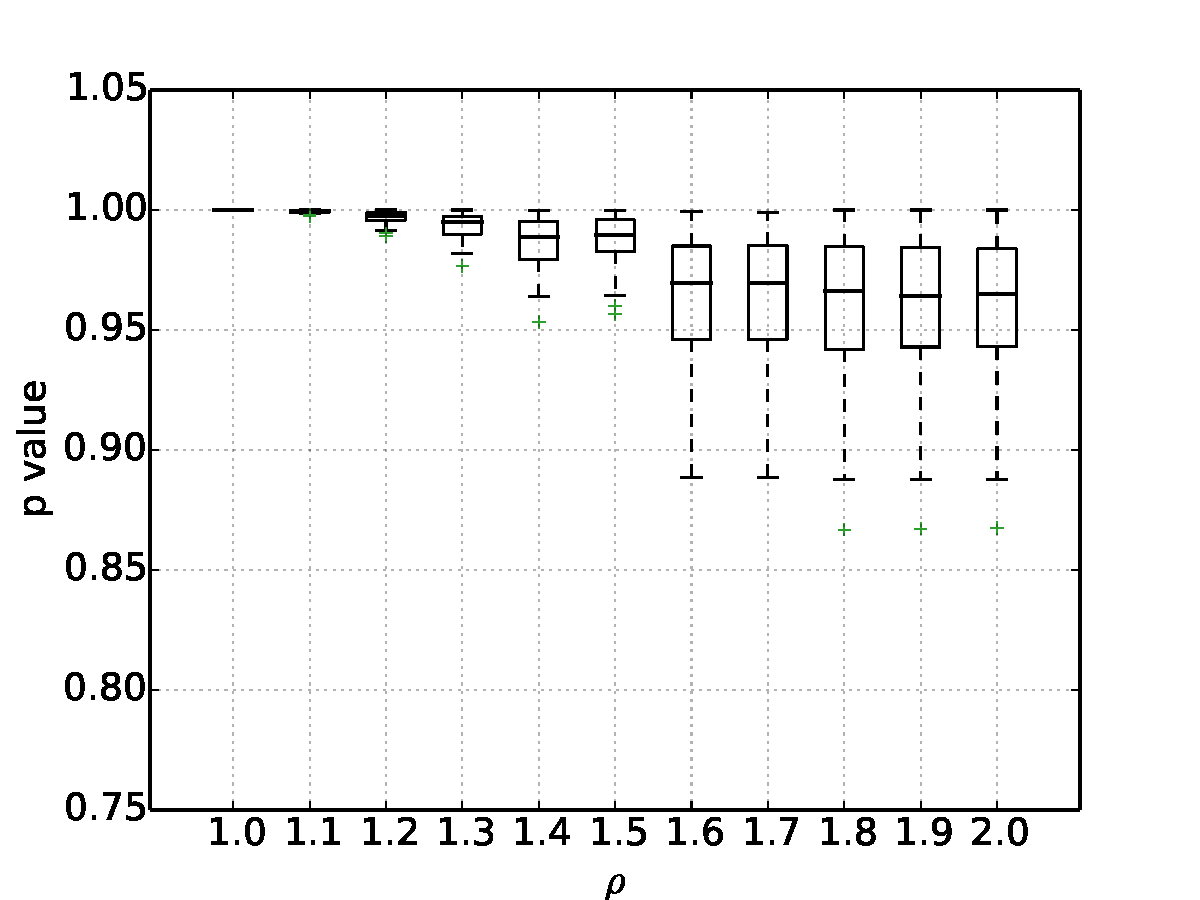
\includegraphics[width=0.49\textwidth]{figs/fig-rho-p-value-rr.pdf}
}
\subfloat[RBP0.5\label{fig-rho-p-value-rbp50}]{%
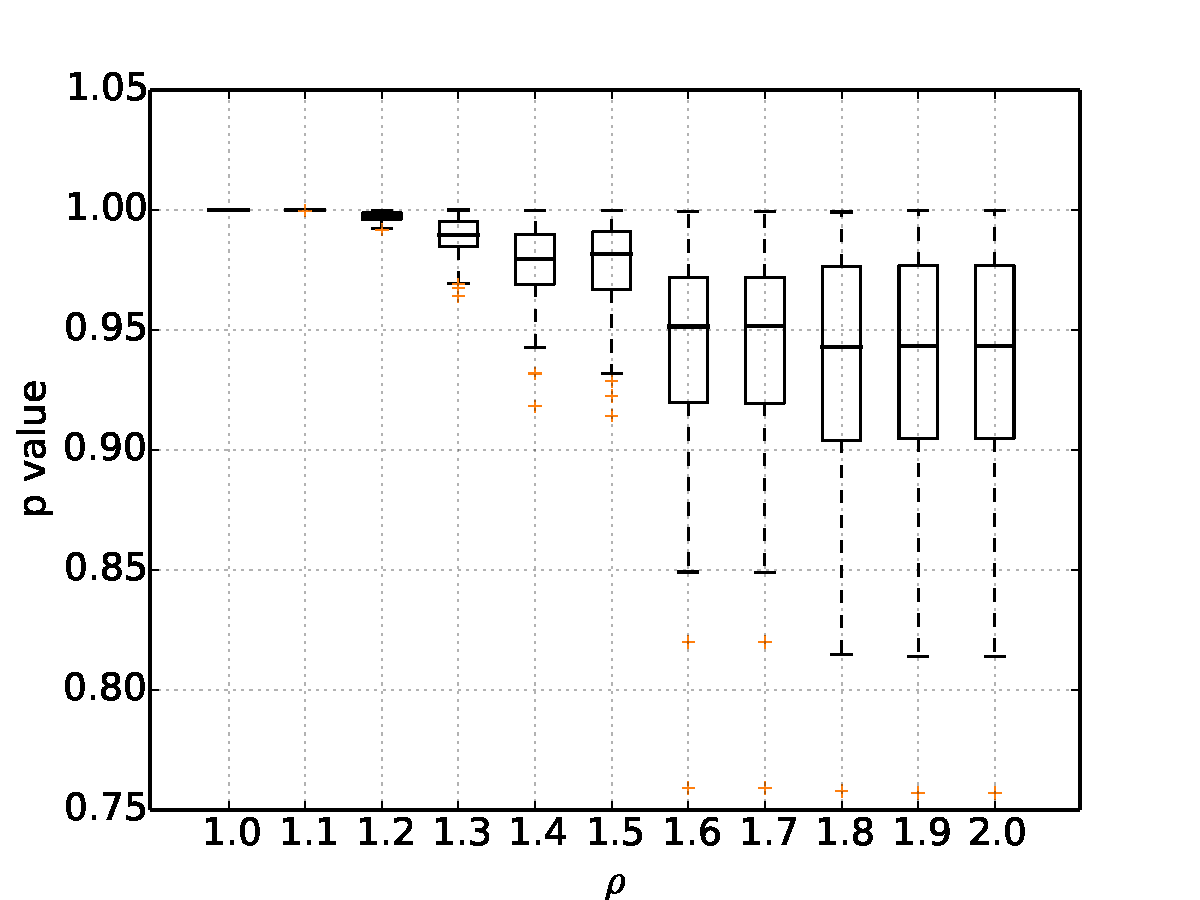
\includegraphics[width=0.49\textwidth]{figs/fig-rho-p-value-rbp50.pdf}
}
\\
\subfloat[RBP0.85\label{fig-rho-p-value-rbp85}]{%
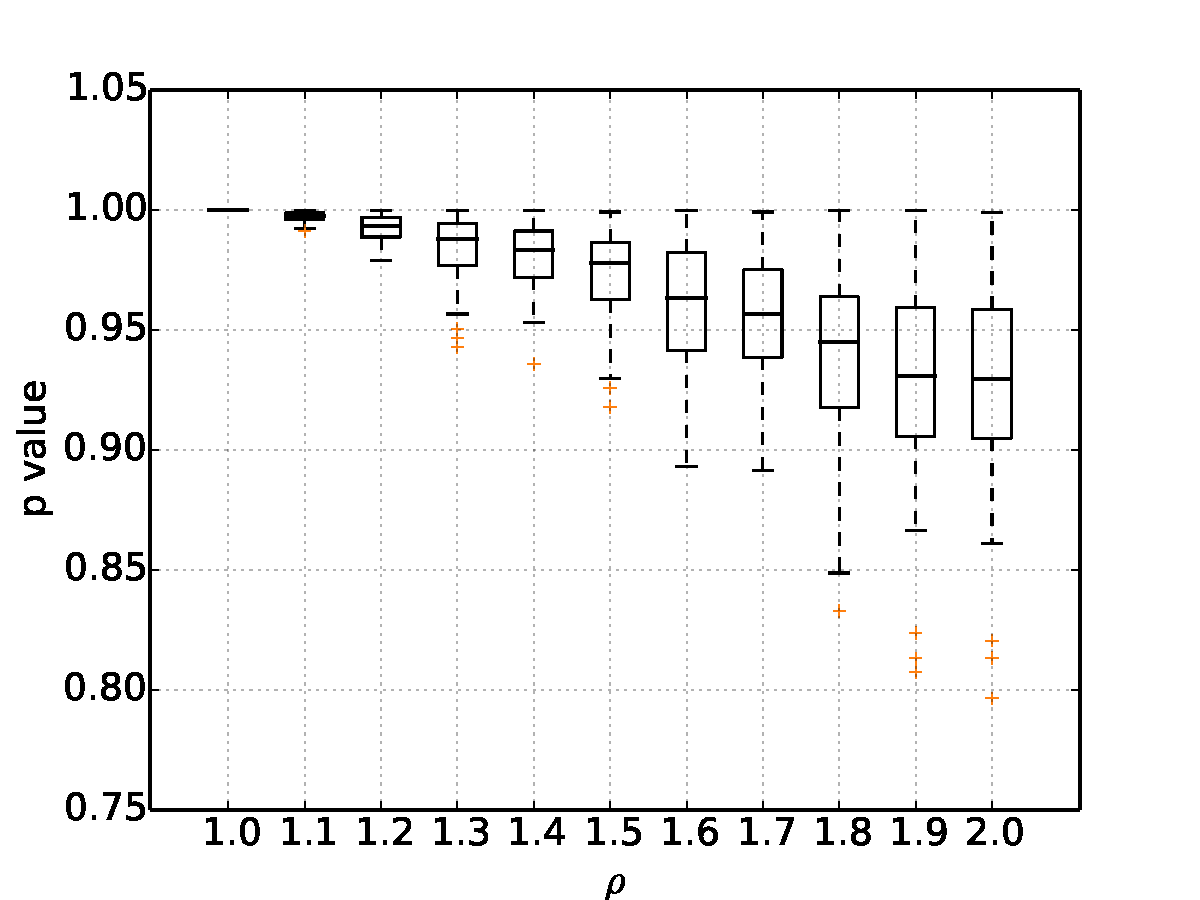
\includegraphics[width=0.49\textwidth]{figs/fig-rho-p-value-rbp85.pdf}
}
\subfloat[AP\label{fig-rho-p-value-ap}]{%
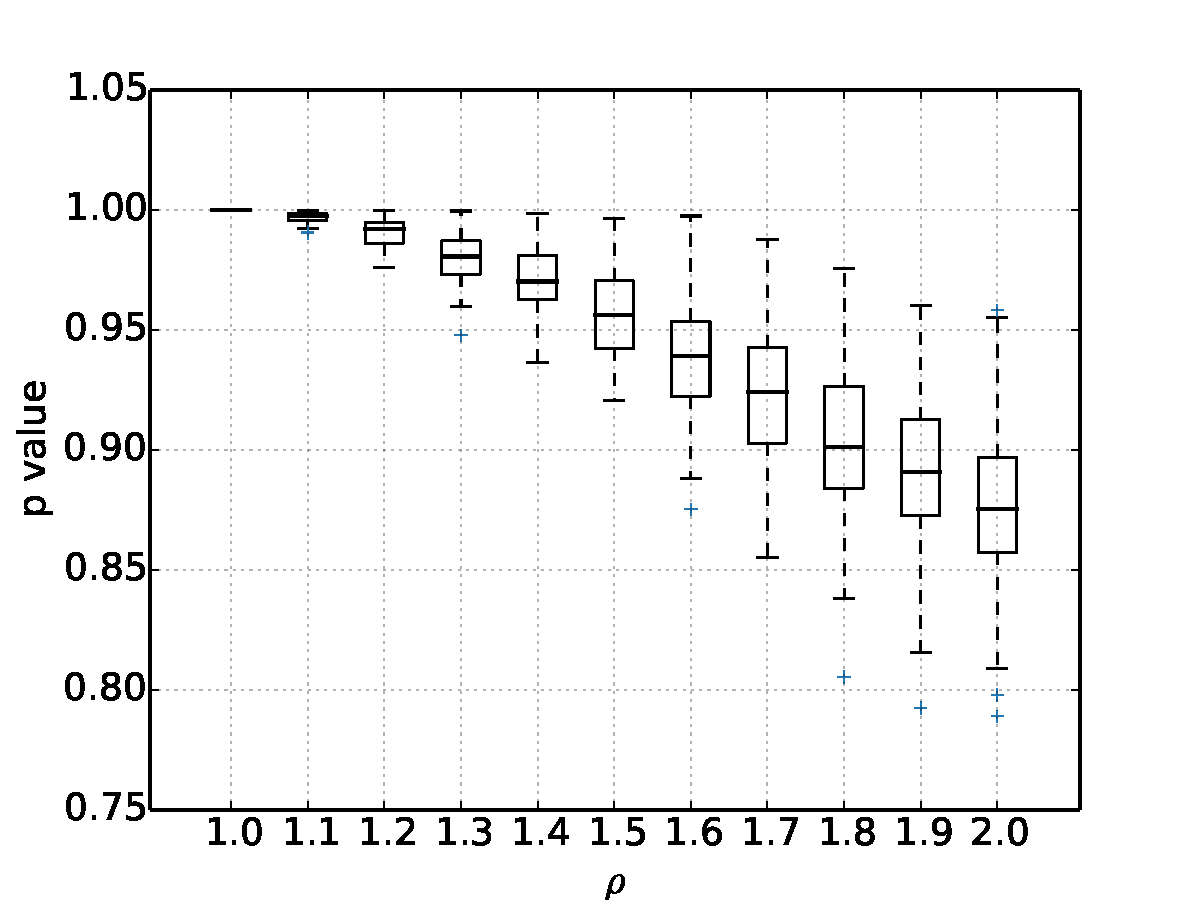
\includegraphics[width=0.49\textwidth]{figs/fig-rho-p-value-ap.pdf}
}
\caption{Distribution of two-tailed $t$-test $p$ values generated by
comparing system scores for $98$ original-order runs, and the
corresponding set of $98$ grouped-score runs ($98$ points plotted in
each column), on each case over a set of $50$ topic scores.
A $p$ value of $1.0$ indicates that the two sets of rankings have
identical means across the $50$ topics.
\label{fig-rho-p-value}}
\end{figure}

Figure~\ref{fig-rho-p-value} explores whether these small score
differences can be regarded as being significant.
To generate the graph, each blocked run was scored for the $50$
topics, and those $50$ per-topic scores used as input to a paired
$t$-test, and compared against the $50$ scores produced in connection
with the ungrouped reference run.
The higher the $p$ value, the more certain it is that the means of
the two alternative approaches -- the reference run, and the grouped
run -- are the same.

As can be seen, {\alistair{more...}}

{\alistair{If don't like the idea of having $p\approx1$ indicating
the two distributions have the same mean, can change tack, and ask
(positive) question is treated run scoring $>0.99$ of original run
scoring.
Then small $p$ values indicate confidence that the treatment achivese
effectiveness within (or greater than) one percent of the original
system.}}

\myparagraph{System Comparison Sensitivity}

Effectiveness measurements are also used to compare systems in a
pairwise manner.
In the second experiment, we explore the implications that score
rounding has on the ability of metrics to differentiate between
systems.
The normal approach to comparing systems is to take their computed
scores across a set of topics, and perform a paired $t$-test to
explore the null hypothesis that the two systems are in fact the
same.
The process of carrying out the $t$-test generates a $p$ value; the
smaller the $p$ value, the smaller the chance that the two systems
being compared are giving the same performance.
To establish significance, a threshold value $\alpha$ is employed,
often $\alpha=0.05$, with $p\le\alpha$ being regarded as a
significant outcome.

\begin{figure}[t]
\centering
\rule{0.5mm}{45mm}
\caption{Variation in $p$ values across system pairs in a set
of runs, plotted as a function of $\rho$, for three different
retrieval effectiveness metrics.
{\alistair{RR, RBP0.85, AP?}}
{\alistair{$\rho = 1.0, 1.1, 1.2, 1.3, \ldots, 2.0$, or something like
that.}}
{\alistair{Box and whisker plot, as $\rho$ is smaller, the mean score
difference should get closer to zero, and the variance should also be
getting smaller.
RR should be relatively unaffected, the others will have broader
variance.
Would be cool in the mean stayed near zero even when $\rho$ is
relatively large.}}
{\alicia{I am sure what should be placed here... have not they all been placed in Figure 2? }}
\label{fig-pair-variation}}
\end{figure}

To measure the effect that score rounding has on system comparisons,
we took the 50 topics of the TREC7 {\todo{citation}} collection
and the 103 runs associated with it, and computed: (a) a set
of $p$ values, generated by comparing each pair of systems using the
metric scores associated with the original set of runs; and then (b)
the corresponding set of $p$ values, generated when the same runs are
first mapped into group scores, and the all-permutations averaging
technique applied.
